
Observacion: \textcolor{red}{(enumerar)} Si en la definic\'ion \textcolor{red}{(recuerdo de mate 1. poner referencia)} (\ref{grafm1}) cambiemos  $A \subseteq \mathbb{R}$ por $A \subseteq \mathbb{R}^{n}$  obtenemos de manera an\'aloga la siguiente definici\'on.    




\begin{definition}  \label{def:grafica}
 
 Sea $f: A\subseteq\Rn{n}\rightarrow\R$; se define la \textit{gráfica de $f$ }, y se nota $graf(f)$,  a
 \[
graf(f)=\{(x_1,x_2,...,x_n,x_{n+1})\in \mathbb{R}^{n+1} \backslash (x_1,x_2,...,x_n) \in A \land f(x_1,x_2,...,x_n)=x_{n+1} \}
 \]


Observaci\'on: \textcolor{red}{Enumerar}   Si $f: A\subseteq\Rn{n}\rightarrow\R$ entonces $graf(f) \subset \mathbb{R}^{n+1}.$
 

Observaci\'on: \textcolor{red}{Enumerar} Dada la  anterio observaci\'onr y con el objetivo de poder dibujar,  nos detendremos especialmente en el caso de gr\'aficas de  campos  $f: A\subseteq\Rn{2}\rightarrow\R,$ cuya definici\'on se desprende automaticamente  de  (\ref{def:grafica}), o sea, el caso
 \[
graf(f)=\{(x,y,z)\in\Rn{3} \backslash (x,y)\subseteq A \land z=f(x,y) \}
 \]



\textcolor{red}{Todo esto va en el recuerdo de mate 1 para completar y corregir los ejemplos------------------------}
\begin{figure}[h!] % El entorno figure te permite incluir imágenes
    \centering
    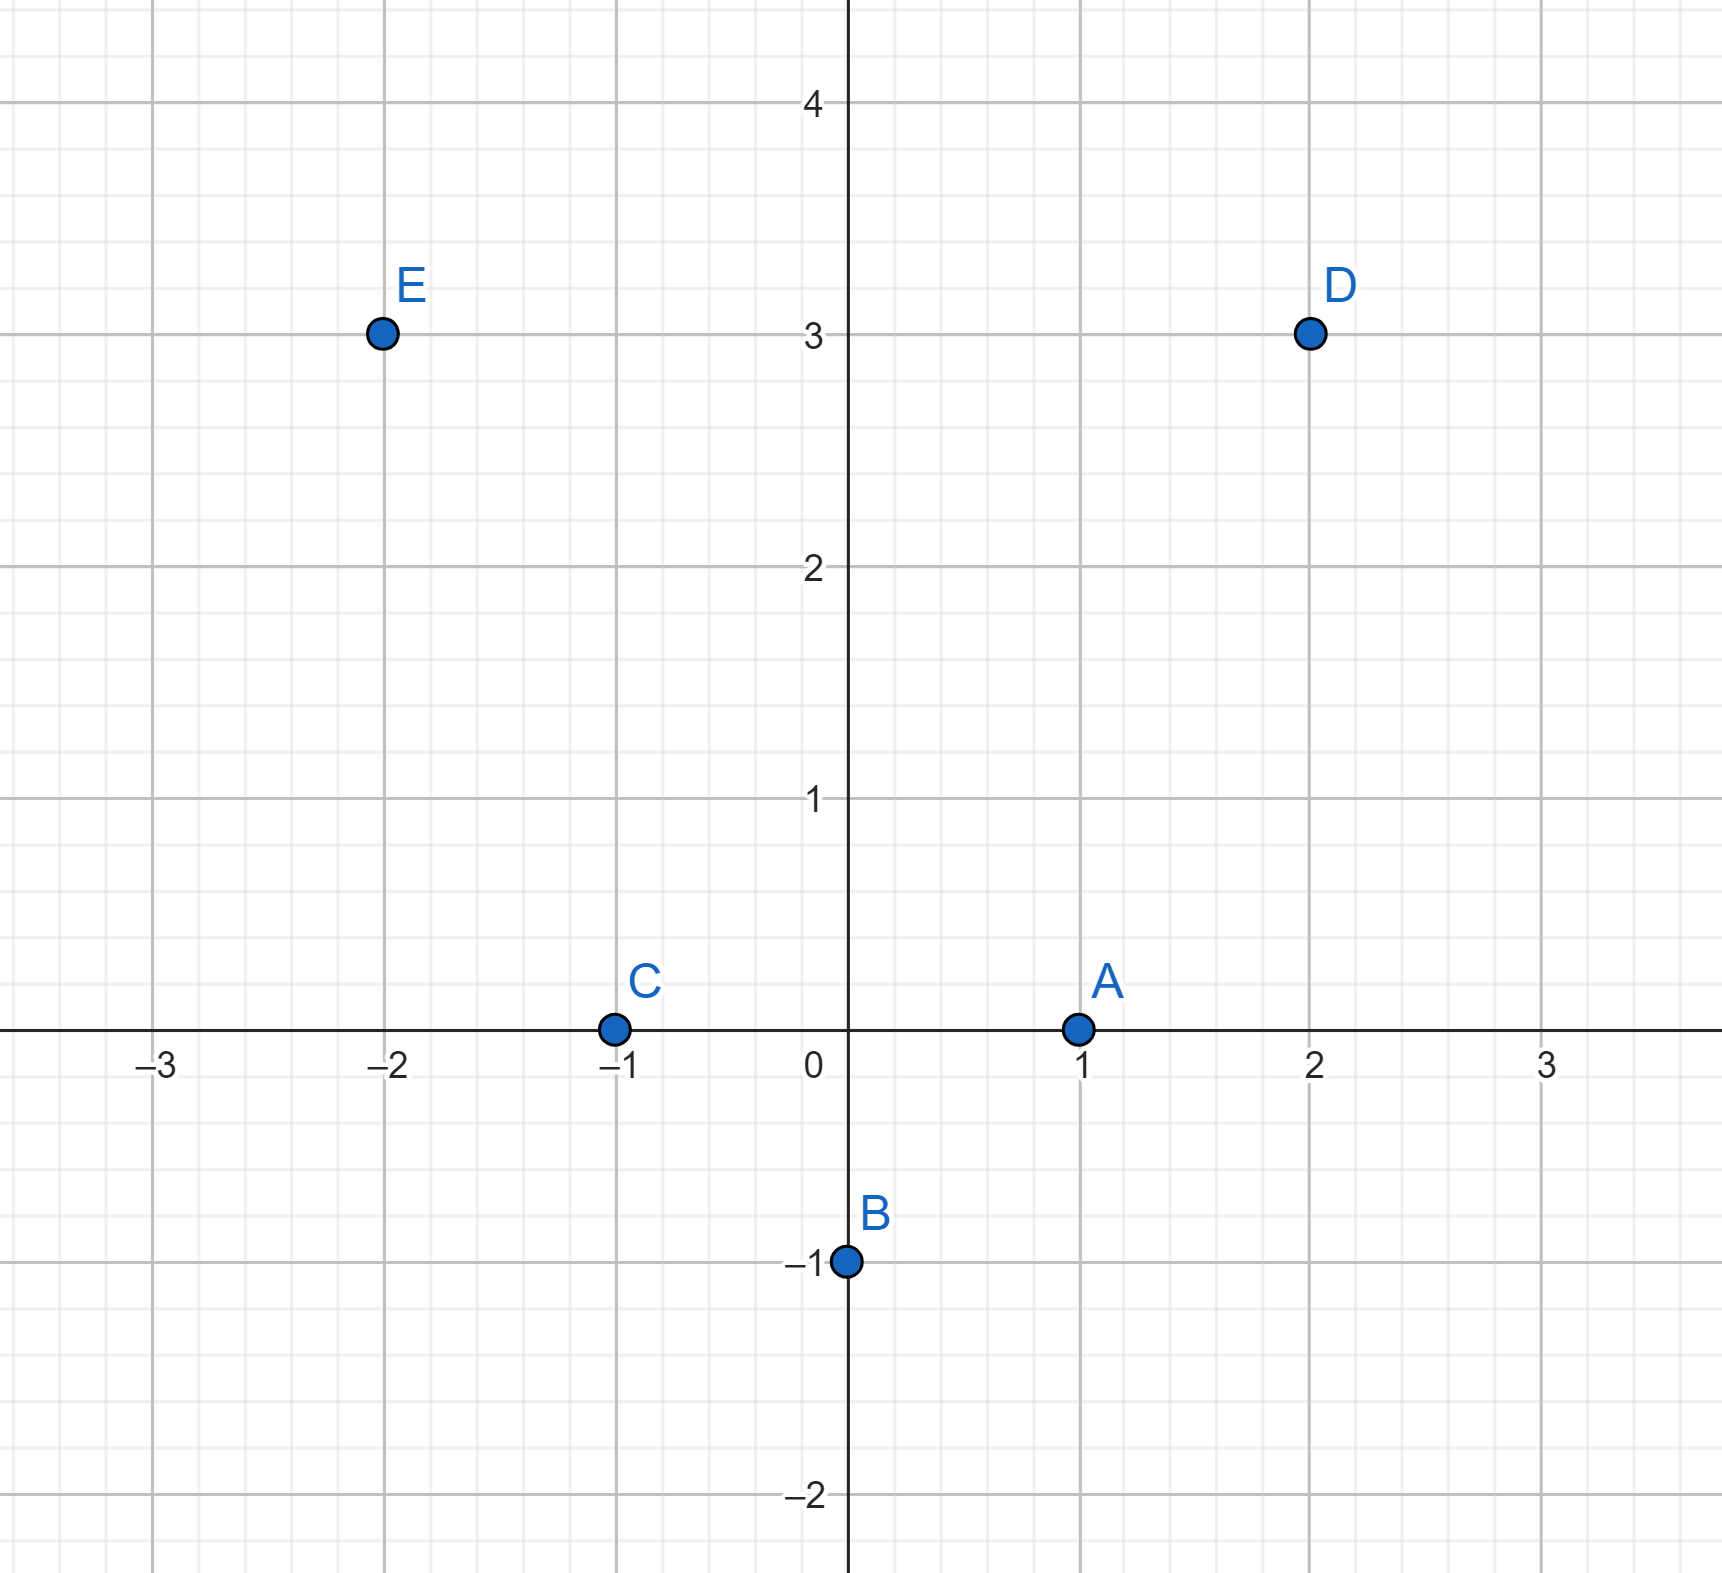
\includegraphics[width=0.34\textwidth]{../figs/Puntos_grafica.png} % Cambia esta ruta por la ubicación de tu imagen
    \caption{Puntos de tabla 1.}
    \label{fig:ejemplo1} % Etiqueta para hacer referencia a la imagen
\end{figure}


De esta manera, se puede empezar a representar la grafica de $f$
\begin{figure}[h!] % El entorno figure te permite incluir imágenes
    \centering
    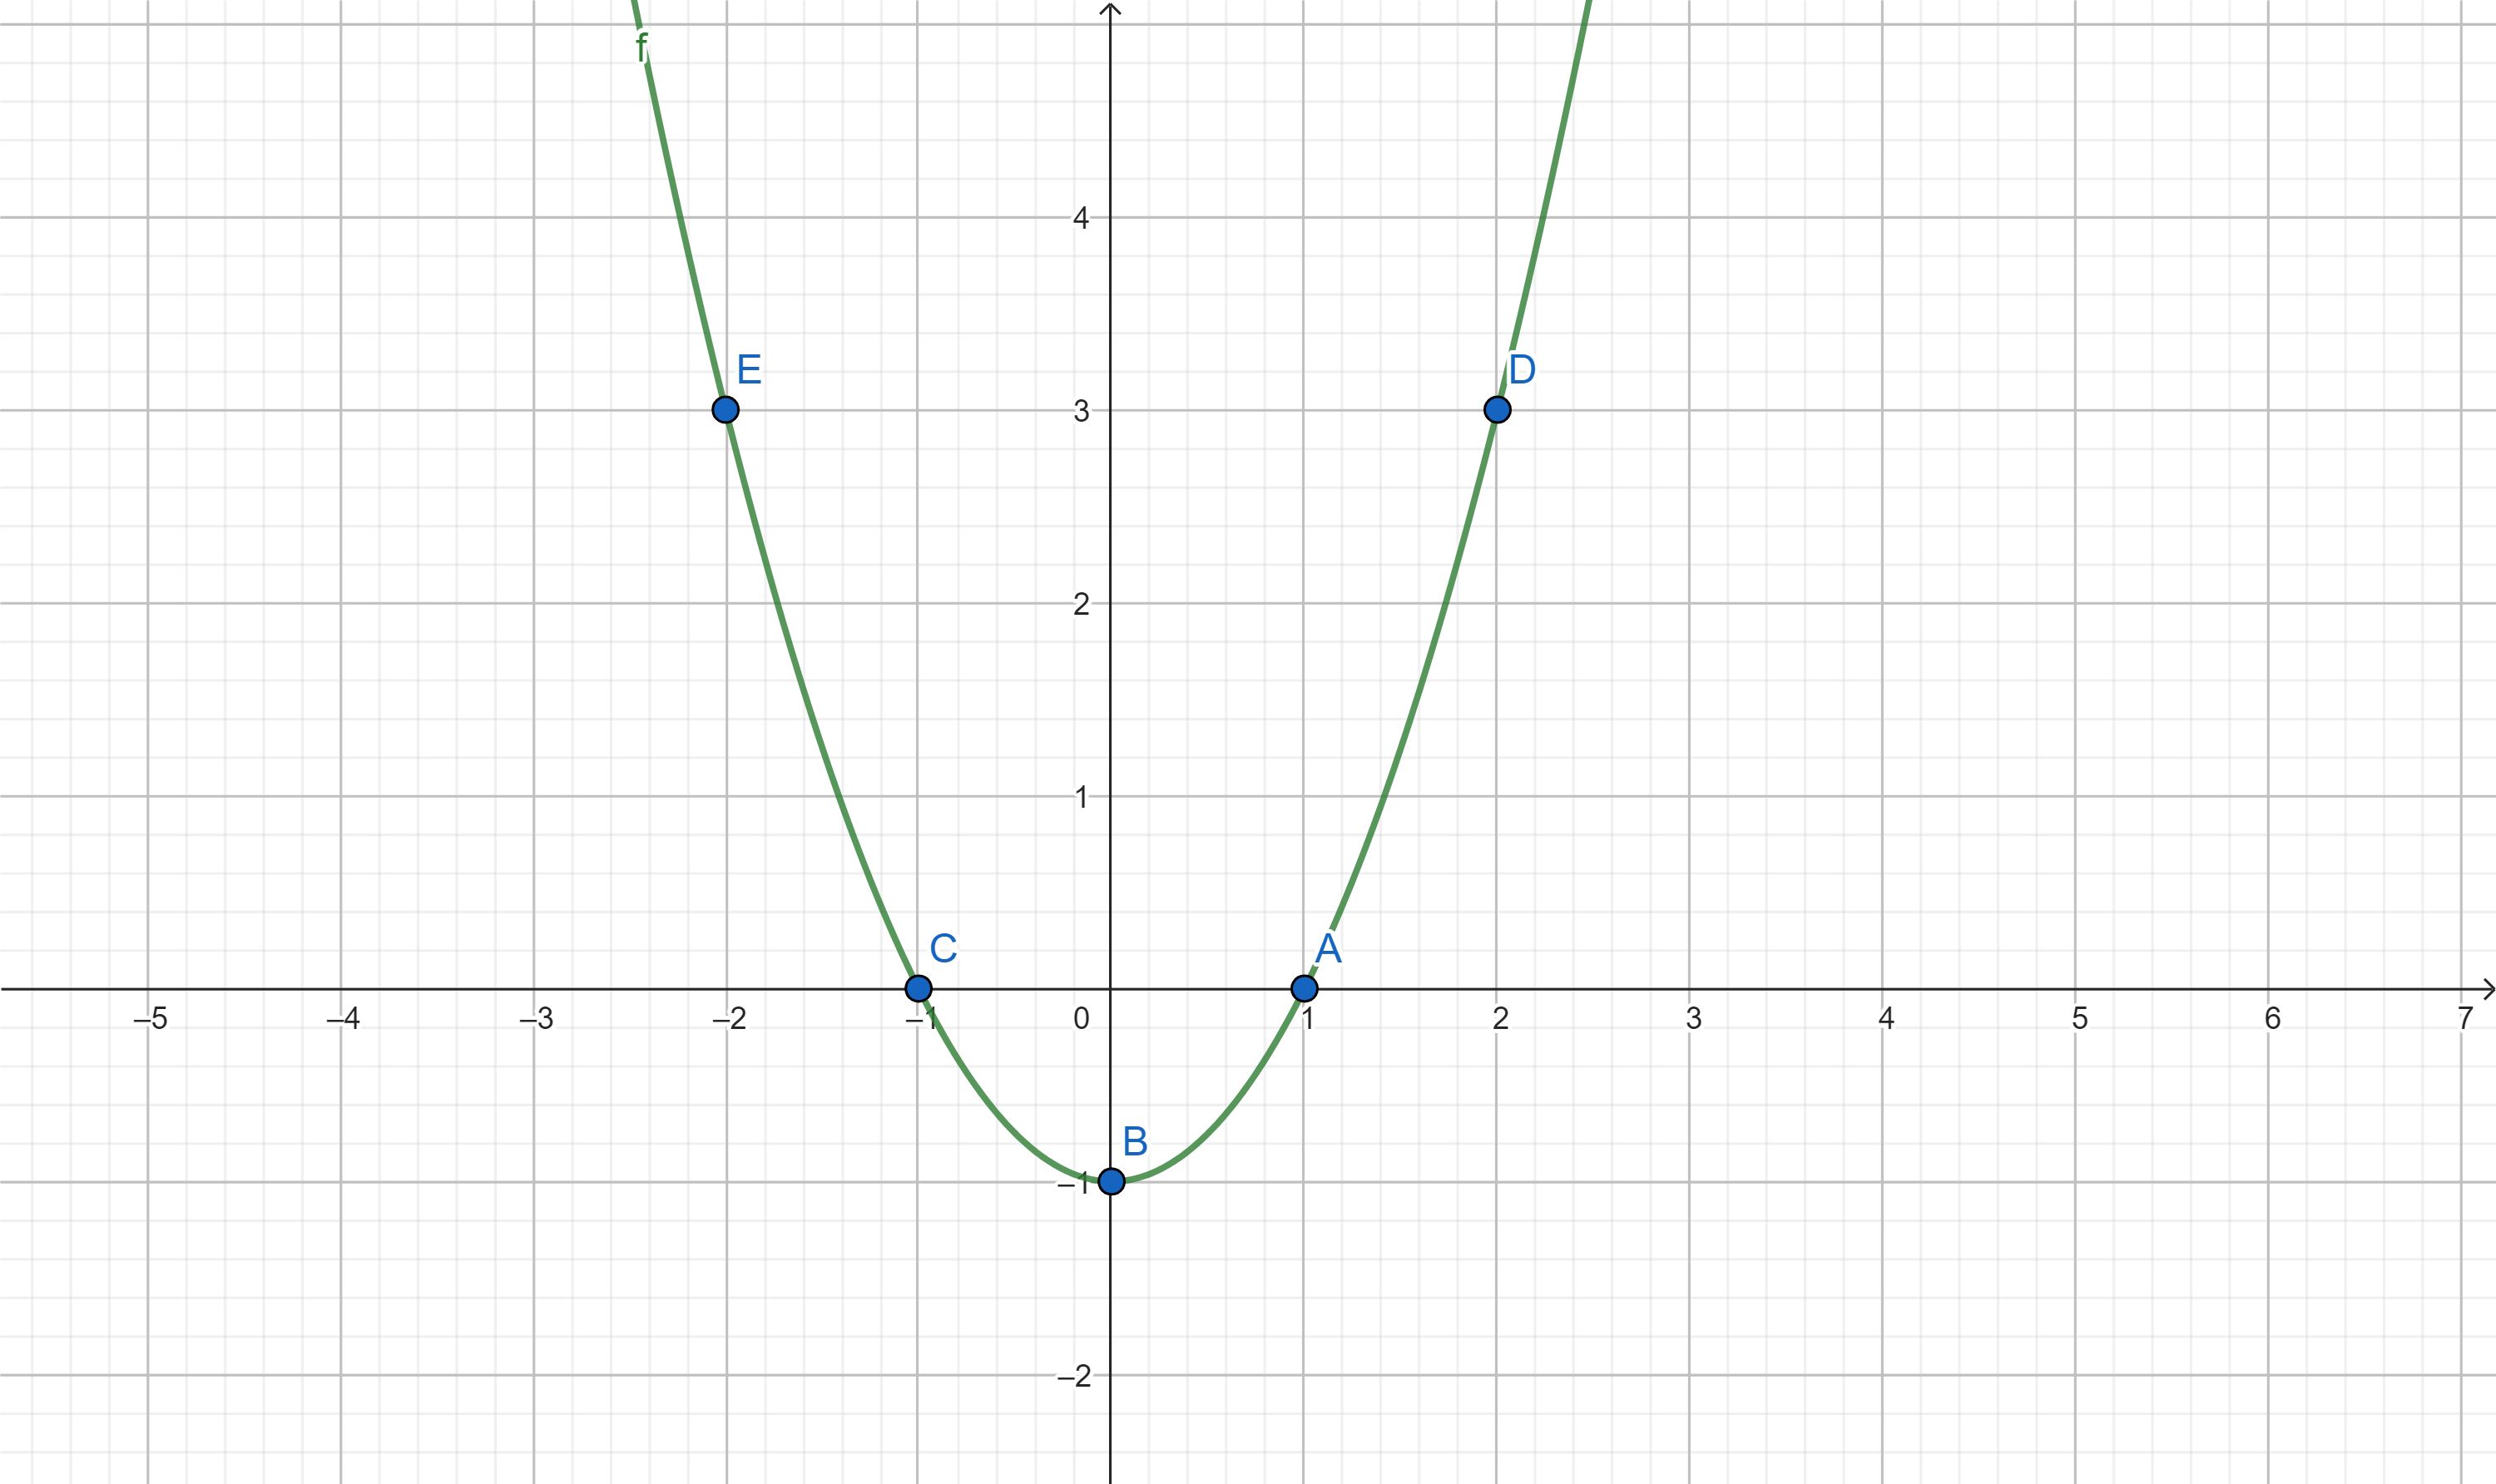
\includegraphics[width=0.5\textwidth]{../figs/r2_grafica.png} % Cambia esta ruta por la ubicación de tu imagen
    \caption{Grafica de $f(x)$.}
    \label{fig:ejemplo2} % Etiqueta para hacer referencia a la imagen
\end{figure}
\end{definition}
\textcolor{red}{Hasta aca---------------------------------------------------------------------------------------------------------}

\vspace{1 cm}

\textcolor{red}{no esta definido conjuntos de nivel --------------------------------------------------------------------------}


En este curso, se analizaran las graficas de funciones en  $\Rn{3}$. Analizamos un ejemplo, tomando $h(x,y)=x^2+y^2$.
Para la función , que representa un paraboloide, los conjuntos de nivel están dados por $h(x,y)=c$, que son círculos concéntricos en el plano xy. Graficando esta función en 3D, podemos ver una superficie parabólica, donde los conjuntos de nivel son las proyecciones de estas circunferencias a diferentes alturas en el eje z y con radio creciente.
\begin{figure}[h!] % El entorno figure te permite incluir imágenes
    \centering
    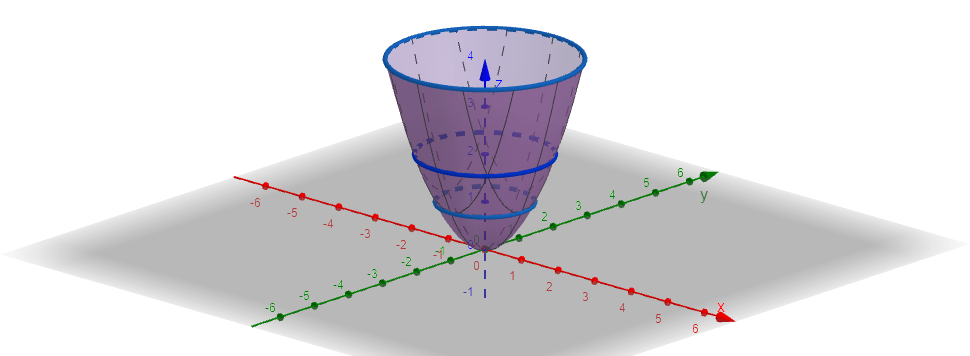
\includegraphics[width=1\textwidth]{../figs/r3_grafica.png} % Cambia esta ruta por la ubicación de tu imagen
    \caption{\small{ Gráfica de h y conjuntos de nivel tomando 
    c=\{1,2,4}\}}
    \label{fig:ejemplo3} % Etiqueta para hacer referencia a la imagen
\end{figure}


\textcolor{red}{Hasta aca---------------------------------------------------------------------------------------------------------}
